\def\probtitle{예시 문제 -- 풍경}
\def\probno{X} % 문제 번호

\begin{problem}{\probno{}. \probtitle{}}

숭실이는 화려하고 특이한 땅으로 유명한 South Dakota Badlands의 사진을 찍기 위해 하루 동안 Rapid City로 여행하기를 결정하였다. 숭실이는 아마추어 사진가이지만 조명 조건에 대해서는 매우 까다롭다.

\begin{center}
    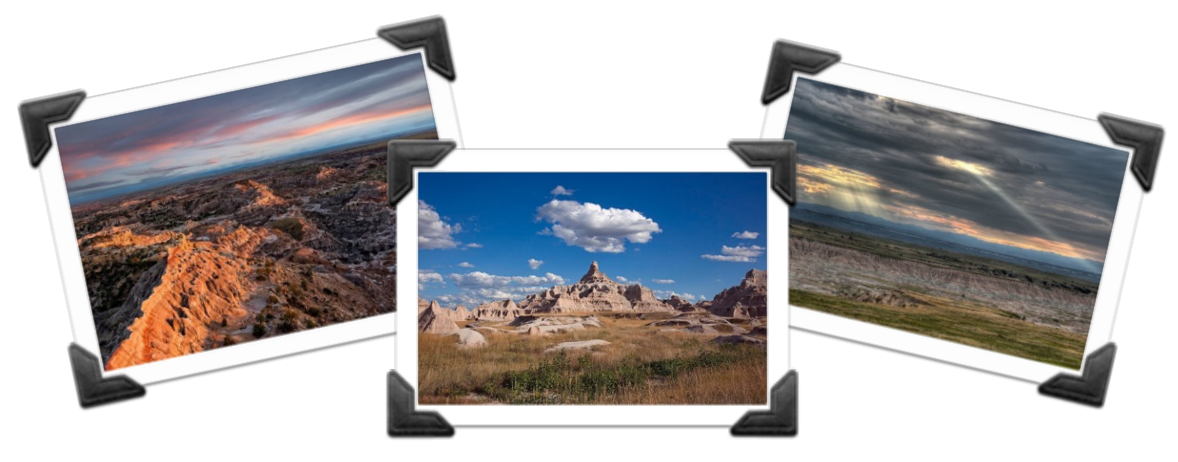
\includegraphics[width=0.5\linewidth]{image/scenery.png}
    
    Images by John Fowler, Carol Highsmith, and Richard Woodland
\end{center}

몇 가지 면밀한 조사를 거쳐 숭실이는 그림 같은 풍경으로 둘러싸여 있는 Badlands의 아름다운 위치를 찾았고, 이 위치에서 촬영하기 위한 다양한 풍경을 정했다.

각 풍경에 대해, 숭실이는 태양의 위치가 이상적인 가장 이른 시각과 가장 늦은 시각을 확인하였다. 삼각대와 카메라를 다시 배치해야 할 필요성과 완성도를 볼 때, 각 사진을 찍기 위해서는 어느 정도의 시간이 필요하고, 이 시간은 정확히 $T$분임이 알려져 있다.

숭실이가 원하는 사진을 모두 찍을 수 있을지 확인하는 프로그램을 작성하라.

\InputFile

첫 번째 줄에 찍고자 하는 사진의 수를 나타내는 정수 $N$과 각 사진을 찍기 위해 필요한 시간을 나타내는 정수 $T$가 주어진다.

이후 $N$개의 줄에는 각 사진을 찍을 수 있는 가장 이른 시각과 가장 늦은 시각을 나타내는 두 정수 $a$와 $b$가 주어진다.

\OutputFile

$N$개의 사진을 모두 찍을 수 있으면 \texttt{yes}, 아니면 \texttt{no}를 출력한다.

\Constraints

\begin{itemize}[topsep=0pt,noitemsep]
    \item $1 \le N \le 10\,000$
    \item $1 \le T \le 100\,000$
    \item $a+t \le b \le 10^9$, $0 \le a, b$
    \item 입력으로 주어지는 수는 모두 정수이다.
\end{itemize}

\Example

\begin{example}
    \exmpfile{./example/01.in.txt}{./example/01.out.txt}%
    \exmpfile{./example/02.in.txt}{./example/02.out.txt}%
\end{example}

입력과 출력을 한 줄에 보여줌

\begin{examplewide}
    \exmpfile{./example/03.in.txt}{./example/03.out.txt}%
\end{examplewide}

여러 줄에 나눠서 보여줌

% \newpage

\Notes

그림은 이렇게 그릴 수 있음

\begin{figure}[!h]
    \centering
    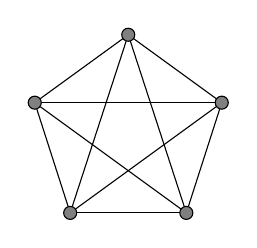
\begin{tikzpicture}[every node/.style={draw, fill=gray, scale=0.5}]
        \def \h {1.25}
        \node[circle] (1) at (0, 1*\h) {};
        \node[circle] (2) at (-0.95*\h, 0.31*\h) {};
        \node[circle] (3) at (0.95*\h, 0.31*\h) {};
        \node[circle] (4) at (-0.59*\h, -0.81*\h) {};
        \node[circle] (5) at (0.59*\h, -0.81*\h) {};
        \draw (1) -- (2);
        \draw (1) -- (3);
        \draw (1) -- (4);
        \draw (1) -- (5);
        \draw (2) -- (3);
        \draw (2) -- (4);
        \draw (2) -- (5);
        \draw (3) -- (4);
        \draw (3) -- (5);
        \draw (4) -- (5);
    \end{tikzpicture}
    \caption{5개의 기둥과 10개의 빔으로 구성된 골조}
\end{figure}

\end{problem}